\section{Detailkonzept} \label{sec:detailkonzept}

Das Konzept mit den Wasserliften ist am besten geeignet für unsere Anwendung. Es existieren bereits solche «Rohrkettenförderer», die jedoch Produkte hinaufbefördern. Wir nutzen dieses System um das Wasser nach unten zu befördern und dabei Energie zu gewinnen. Es werden insgesamt sechs Lifte benötigt. Fünf Lifte überwinden je 60.08\si{m} und der unterste Lift überwindet 80.24\si{m}. In der Abbildung \ref{fig:PrinzipGrobkonzept4} \nameref{fig:PrinzipGrobkonzept4} ist dies grafisch dargestellt.

\subsection{Elektronik}

\paragraph{Generator}
\begin{figure}[H]
\centering
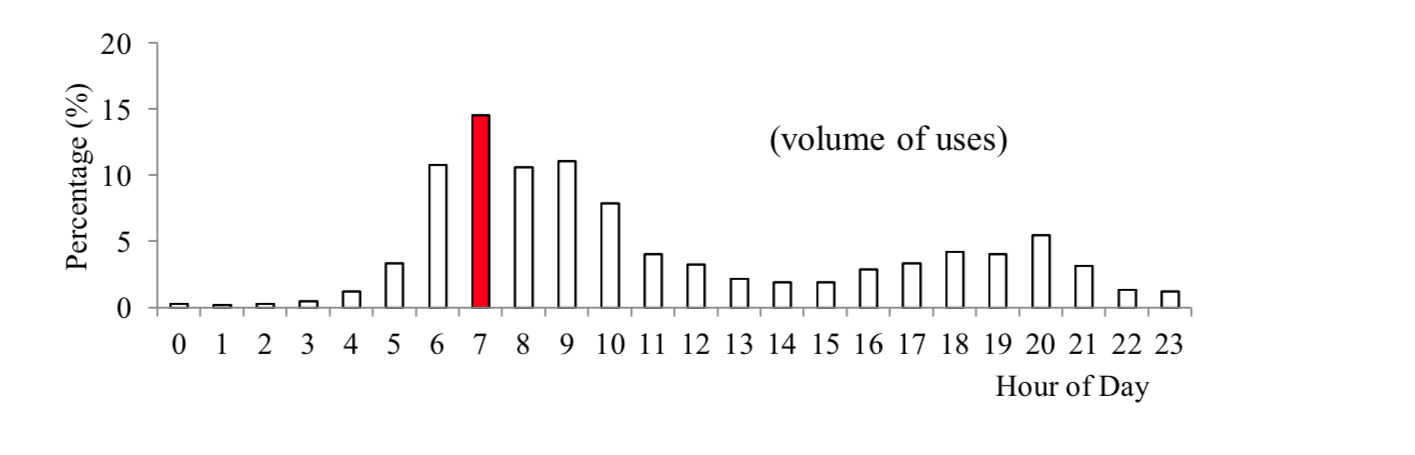
\includegraphics[width=\linewidth]{tagesGangKurve.png}
\caption{Typische Tagesgangkurve. \cite{peakWaterDemand}}
\label{fig:tagesGangKurve}
\end{figure}
\paragraph{Anzeige}

\subsection{Mechanik}

\paragraph{Abflussrohr}

\paragraph{Rohrkette}


\subsection{Kosten}